\documentclass[a4paper]{article}
\usepackage[letterpaper, margin=1in]{geometry} % page format
\usepackage{listings} % this package is for including code
\usepackage{graphicx} % this package is for including figures
\usepackage{amsmath}  % this package is for math and matrices
\usepackage{amsfonts} % this package is for math fonts
\usepackage{tikz} % for drawings
\usepackage{hyperref} % for urls
\usepackage[section]{placeins}
\usepackage{float}

\title{Homework 0}
\author{Alex Shah}
\date{9/7/16}

\begin{document}
\lstset{language=Python}

\maketitle

\section{Python Proof 2.1}
\subsection{Python Installation Proof and Output}
\lstinputlisting[language=Python,frame=single]{2-1.py}
Output:
\lstinputlisting[language=Python,frame=single]{2-1results.txt}

\clearpage

\section{Github Proof 2.2}
\subsection{Github Collaborators}
\begin{figure}[H]
  
\includegraphics[width=\textwidth]{2-2-gitProof.png}  
\end{figure}

\clearpage

\section{Kaggle Proof 2.3}
\subsection{Kaggle Account Page}
 \begin{figure}[H]
  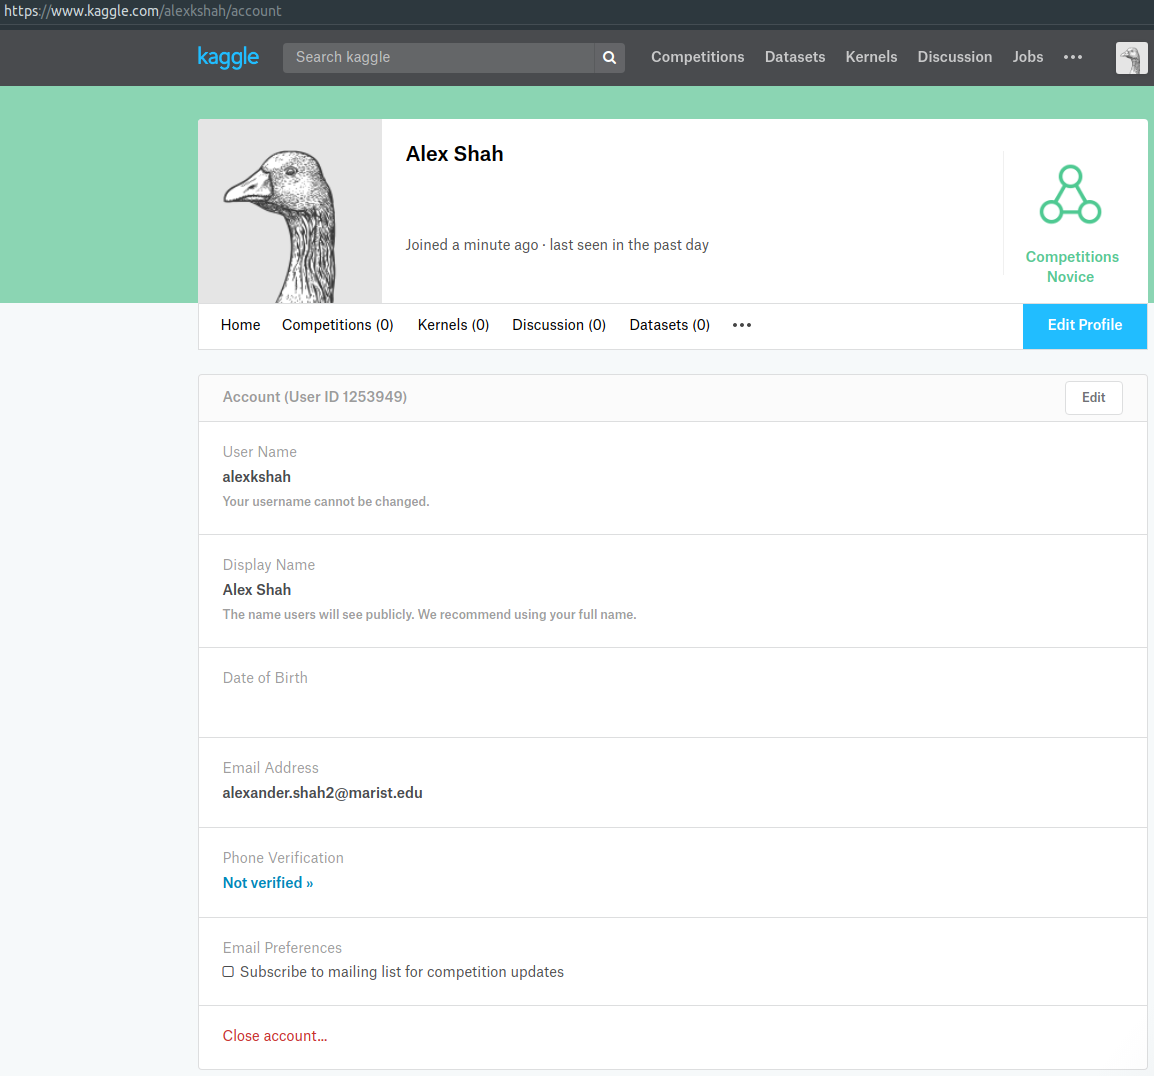
\includegraphics[width=\textwidth]{2-3-kaggleProof.png}  
\end{figure}

\clearpage

\section{Problems}
\subsection{}
This problem was solved using Scipy's fmin function, inverted to produce a maximum. The answer is 4.

\lstinputlisting[language=Python,frame=single]{4-1.py}

\subsection{}
Using x and y for readability, the partial derivative of f(x) with respect to x:
\begin{equation}
f(x)=3x^3-3xy^2+4y-8
\end{equation}
\begin{equation}
3*3*x^2-3*y^2+4*0-0
\end{equation}
\begin{equation}
9x^2-3y^2
\end{equation}
The partial derivative of f(x) with respect to y:
\begin{equation}
f(x)=3x^3-3xy^2+4y-8
\end{equation}
\begin{equation}
3*0-3x*2y+4*1-0
\end{equation}
\begin{equation}
6xy+4
\end{equation}

\clearpage

\subsection{}
\lstinputlisting[language=Python,frame=single]{4-3.py}

\clearpage

Output:

\lstinputlisting[language=Python,frame=single,breaklines=true]{4-3Results.txt}

\subsection{}
$X \sim N(2,3)$

X is a random variable.

N(2,3) shows that the normal distribution has a mean, $\mu$, of 2.

And a variance denoted as $\sigma^{2}$ which gives us $\surd 3$ for $\sigma$.

In a normal distribution, the expected value is the mean (in this case 2) with a variance of $\surd 3$. 

Using these values, we can expect X within the range :
  \begin{equation}
  \mu - \sigma \leq X \leq \mu + \sigma
  \end{equation}
or
  \begin{equation}
  2 - \surd 3 \leq X \leq 2 + \surd 3
  \end{equation}

for 1 standard deviation from the mean, or expected value. 

Or within 2 standard deviations 
  \begin{equation}
  2 - 2 * \surd 3 \leq X \leq 2 + 2 * \surd 3
  \end{equation}

\end{document}
